\documentclass{article}
\usepackage{graphicx}

\begin{document}

\title{Documentação do PI}
\author{Kauê José Abdalla Leal}
\date{03/04/2024}

\maketitle

\begin{center}
      Izabela Tayná Reis Coimbra (PO)

      Kauê José Abdalla Leal (Design e Documentação)

      Isabela Maria de Oliveira (Back-End)

      Pedro Victor Virgino da Cunha (Front-End)

      Victor Ferreira Neves (Front-End e Back-End)
\end{center}


\section{Briefing}
Viajar, para muitos, é uma experiência transcendental, um momento de descoberta e aventura. No entanto, por trás da maravilha das paisagens exóticas e dos sorrisos em fotos, existe uma jornada de planejamento muitas vezes árdua e complexa. É nesse cenário desafiador que nasce nosso projeto: uma plataforma inovadora voltada para o planejamento de viagens, compartilhamento de experiências e dicas de economia.
Nossa história é moldada por diversos atores, cada um com seu papel único. Temos os viajantes individuais, sedentos por aventura e novas descobertas. Os grupos de viajantes, unidos pelo espírito de camaradagem e pela busca de experiências compartilhadas. E, é claro, nossa comunidade online de viajantes, o coração pulsante dessa jornada coletiva. O dilema é universal: escolher destinos, estimar custos, montar itinerários e enfrentar a barreira linguística são apenas alguns dos obstáculos que os viajantes enfrentam. Nosso propósito é simplificar essa jornada, oferecendo uma solução centralizada e confiável.
A jornada do viajante está repleta de desafios que demandam soluções digitais inteligentes. Desde o desenvolvimento de uma plataforma centralizada de planejamento de viagens até a agregação de informações confiáveis, cada etapa do processo é uma oportunidade para criar valor para nossa comunidade. Facilitar o compartilhamento de experiências, construir e manter uma comunidade global de viajantes e explorar oportunidades de monetização são áreas que exigirão foco e inovação para alcançar o sucesso. O coração do nosso projeto reside em uma plataforma online, meticulosamente desenvolvida para abrigar todas as necessidades do viajante moderno. Aqui, é possível pesquisar destinos, obter estimativas de custos, organizar itinerários e até mesmo facilitar a comunicação em terras estrangeiras. Tudo isso em um único lugar, com acesso fácil e intuitivo.
Nossa escolha pela área de negócio do turismo e viagens é respaldada por uma série de justificativas sólidas. A demanda crescente por soluções de planejamento de viagem acessíveis e confiáveis é evidente em um mundo onde viajar se torna cada vez mais acessível. O aumento do número de viajantes independentes e de baixo orçamento clama por uma plataforma que atenda às suas necessidades específicas. Além disso, reconhecemos a importância da comunidade e do compartilhamento de experiências na tomada de decisões de viagem, um aspecto que será fundamental em nosso projeto. E, por fim, a oportunidade de monetização através de parcerias e publicidade direcionada garante não apenas a sustentabilidade financeira da plataforma, mas também a entrega de valor adicional aos nossos usuários.

\section{Plano 5WH1}

\begin{enumerate}
      \item O que é o problema? (What)

            O processo de planejamento de viagem é complexo e desafiador para muitos viajantes. Eles enfrentam dificuldades ao escolher destinos, estimar custos, organizar itinerários e se comunicar em ambientes estrangeiros.
      \item Por que o problema ocorre? (Why)

            O problema ocorre devido à falta de acesso a informações confiáveis, dificuldade em compartilhar experiências de viagem e a necessidade de conectividade com uma comunidade global de viajantes.
      \item Quem são as pessoas que vivem o problema? (Who)

            Viajantes individuais, grupos de viajantes e a comunidade online de viajantes são os principais atores envolvidos.
      \item Onde as pessoas que vivem o problema estão? (Where)

            Os viajantes enfrentam esse problema em todas as etapas do processo de planejamento de viagens, desde a escolha do destino até a execução do itinerário em um ambiente estrangeiro.
      \item Quando o problema acontece? (When)

            O problema ocorre sempre que os viajantes estão planejando, organizando ou executando suas viagens, especialmente quando enfrentam dificuldades de logística, comunicação ou seleção de atividades.
      \item Como o problema acontece? (How)

            O problema surge devido à falta de acesso a informações confiáveis, à dificuldade de comunicação em ambientes estrangeiros e à ausência de uma comunidade online para compartilhar experiências e dicas.

\end{enumerate}

\section{Personas}

\begin{itemize}
      \item[$\bullet$] Viajantes Individuais
      \item[] Estes são indivíduos que buscam aventura e novas descobertas através de viagens.
            Eles podem ter diferentes faixas etárias, interesses e orçamentos, mas compartilham uma paixão por explorar o desconhecido.
            Suas necessidades incluem informações detalhadas sobre destinos, dicas de economia, itinerários personalizados e suporte durante a viagem.
      \item[$\bullet$] Grupos de Viajantes
      \item[] Este grupo é composto por amigos, famílias ou colegas que viajam juntos em busca de experiências compartilhadas e camaradagem.
            Eles podem precisar de recursos específicos para planejar viagens em grupo, como opções de hospedagem para grupos grandes, atividades adequadas para diferentes idades e preferências, e ferramentas para coordenar itinerários.
      \item[$\bullet$] Comunidade Online de Viajantes
      \item[] Esta é a comunidade virtual de usuários da plataforma, composta por viajantes individuais e grupos que interagem, compartilham experiências e dicas.
            Eles desempenham um papel crucial na geração de conteúdo gerado pelo usuário, fornecendo avaliações, recomendações e feedback.
            Sua participação é essencial para a construção de uma base de conhecimento confiável e atualizada sobre destinos, acomodações, atividades e muito mais.
            \vspace{\baselineskip}
            \vspace{\baselineskip}
      \item {\subsection {Outras Personas}}
      \item[] Hotéis
      \item[] Companhias Aéreas
      \item[] Agências de Turismo
      \item[] Anunciantes Interessados
\end{itemize}

\section{Matriz CSD}

\begin{figure}[h]
      \centering
      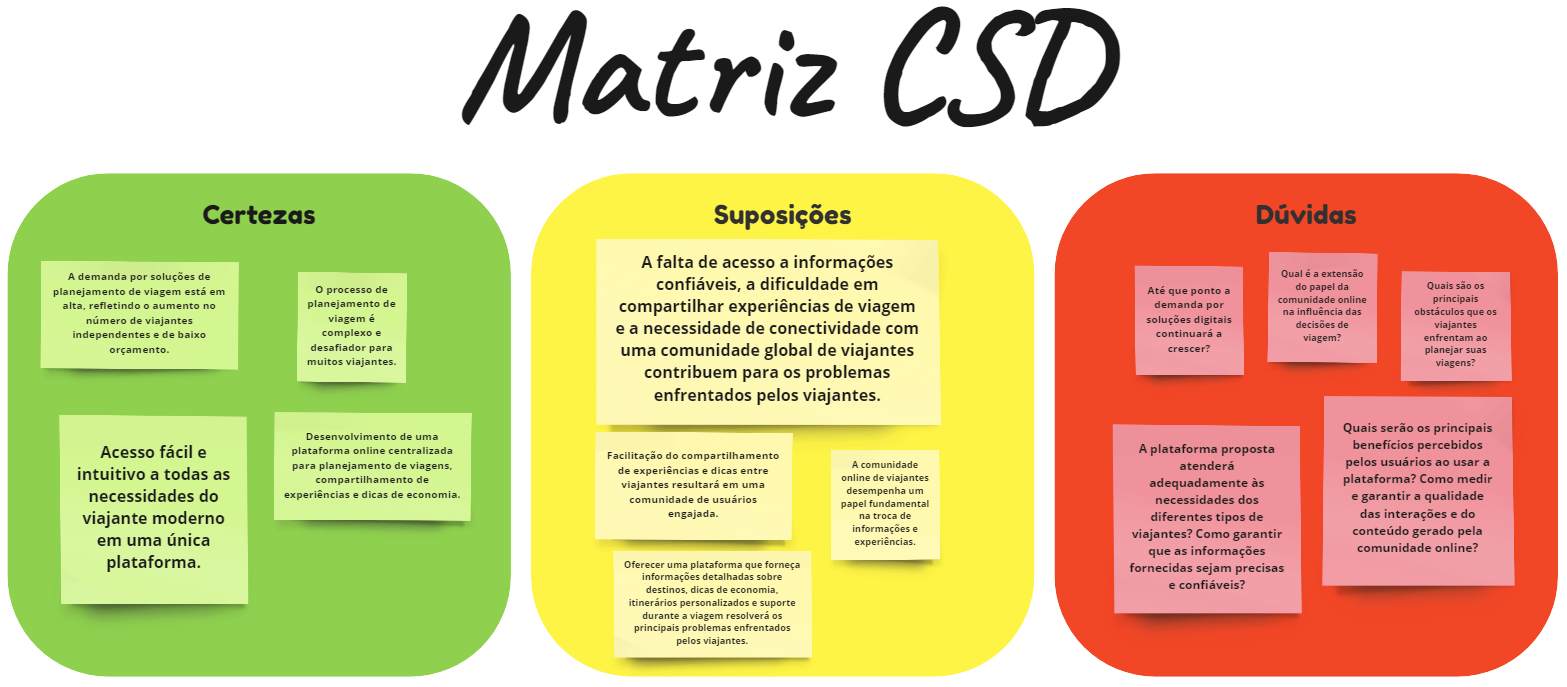
\includegraphics [width=0.6\textwidth]{IMGDOC/Matriz CSD.png}
      \label{fig:imagem}
\end{figure}

\section{Benchmark}
De acordo com pesquisas feitas em sites e redes sociais, os concorrentes tem dificuldades em alguns aspectos, trivago e mochileiros.com não postam muito em suas redes sociais.
Trivago tem problemas com o desempenho de seus sites, já mochileiros.com tem problemas com o desempenho e com sua acessibilidade em seu site.

\subsection{Exemplo Trivago}

\begin{figure}[h]
      \centering
      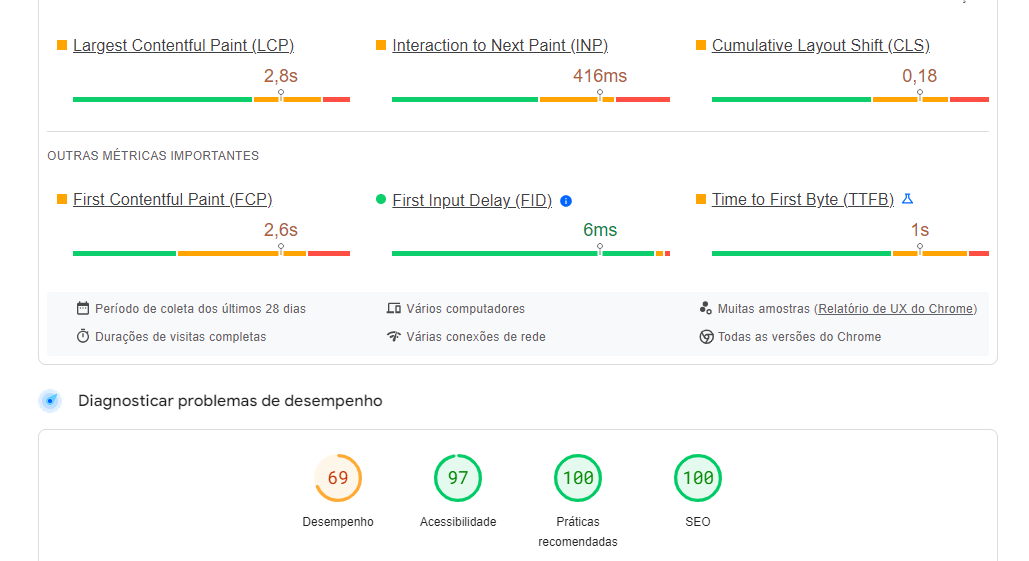
\includegraphics [width=1\textwidth]{IMGDOC/AnaliseTrivago1.png}
      \label{fig:imagem}
\end{figure}
\begin{figure}[h]
      \centering
      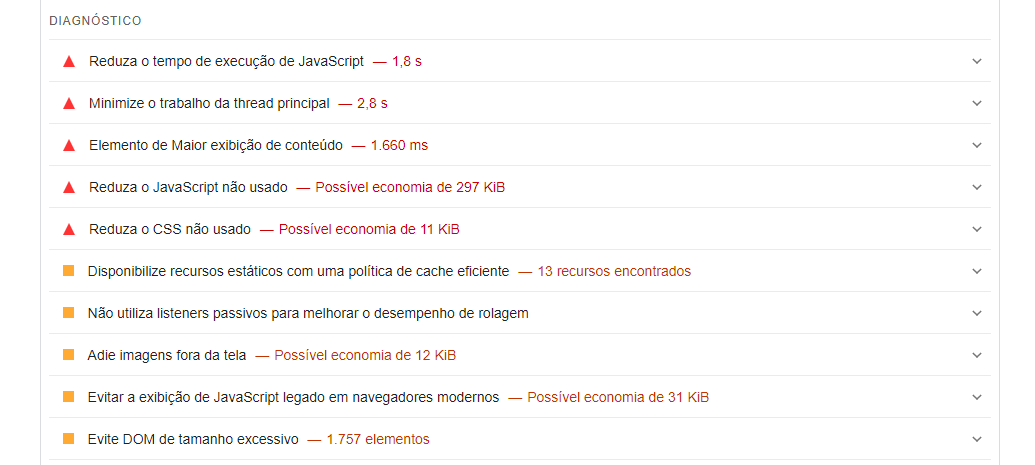
\includegraphics [width=1\textwidth]{IMGDOC/AnaliseTrivago2.png}
      \label{fig:imagem}
\end{figure}

\subsection{Exemplo Mochileiros.com}

\begin{figure}[h]
      \centering
      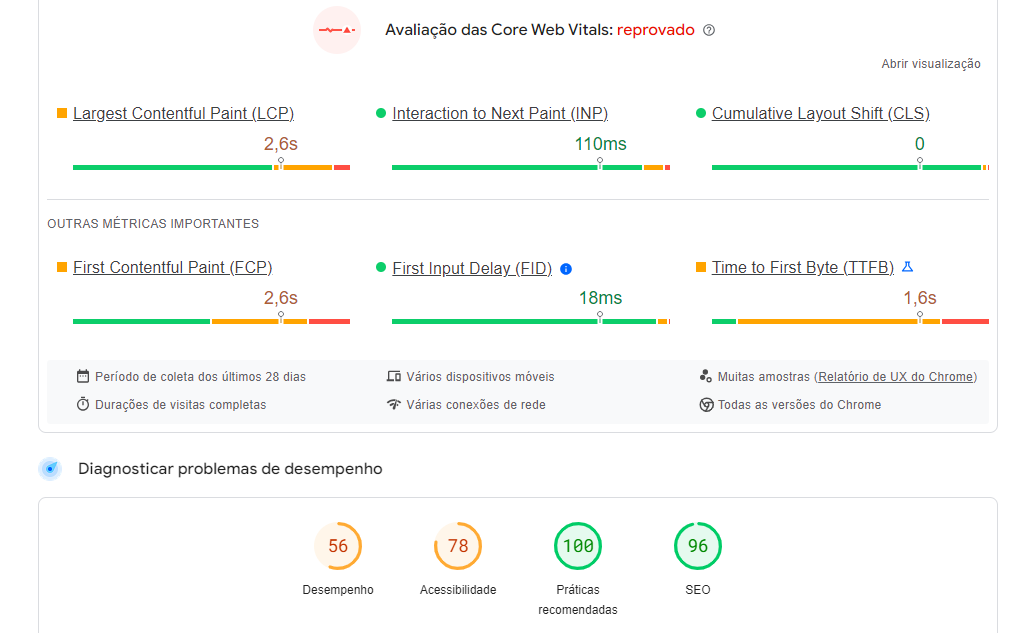
\includegraphics [width=1\textwidth]{IMGDOC/AnaliseMochileiros1.png}
      \label{fig:imagem}
\end{figure}
\begin{figure}[h]
      \centering
      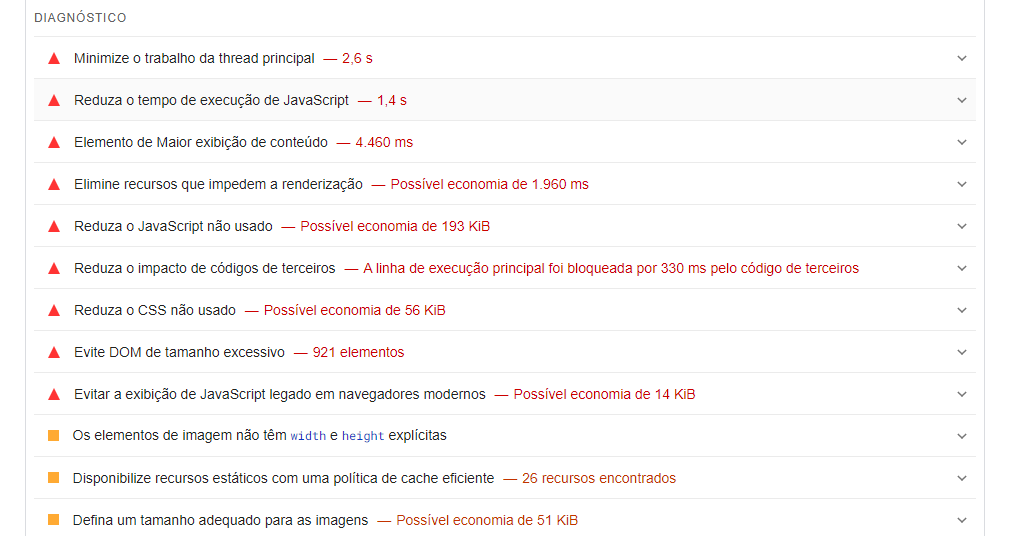
\includegraphics [width=0.9\textwidth]{IMGDOC/AnaliseMochileiros2.png}
      \label{fig:imagem}
\end{figure}

\section{Mapa da jornada do usuário}

\end{document}
